Nieopodal wioski, w której gracz rozpoczął grę znajduje się postać budowniczego. Po podejściu do niego okazuje się, że
można z nim porozmawiać. Jak wskazuje pole dialogowe nazywa się on Rhodan i potrzebuje pomocy. Zapytany w czym trzeba mu
pomóc, prosi gracza o pomoc w wybudowaniu schronienia, gdyż w ostatnim czasie stracił cały swój dobytek w pożarze i
teraz nie ma gdzie mieszkać.

\begin{figure}[h!]
    \centering
    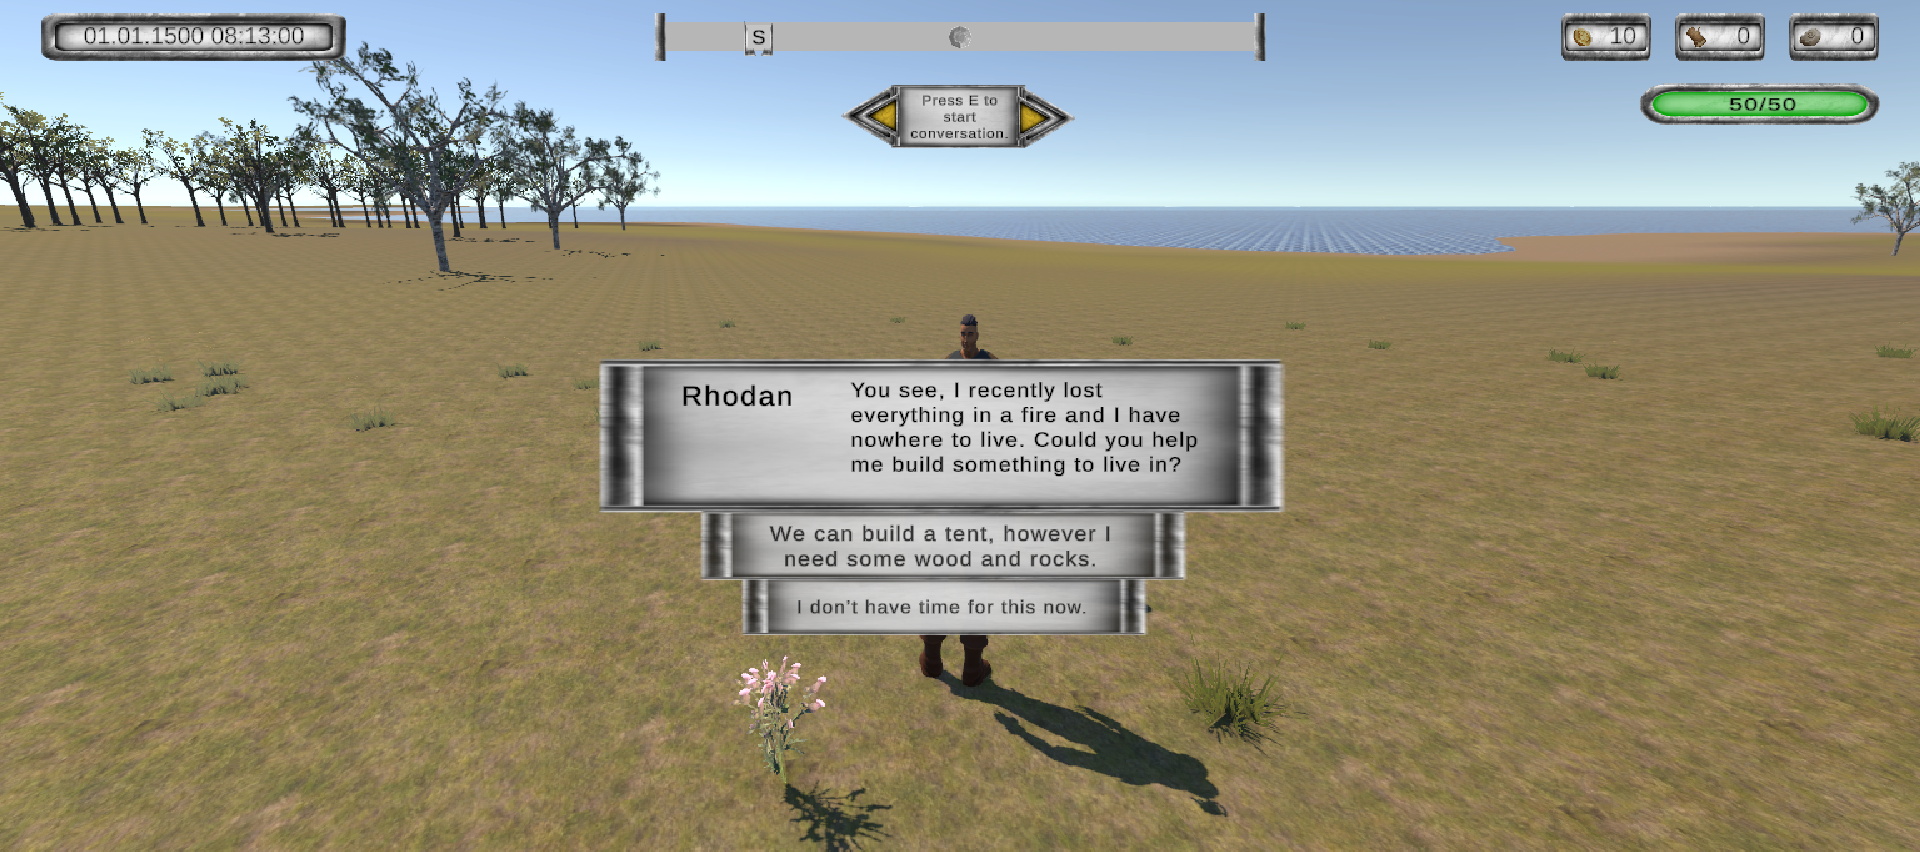
\includegraphics[width=1\textwidth]{images/rozgrywka/rhodan3.png}
    \caption{Kadr z dialogu z Rhodanem podczas którego opowiada swoją historię.}
\end{figure}

Gracz proponuje mu wybudowanie namiotu, jednakże wymaga to zasobów, których nie posiada. Zapytawszy Rhodana gdzie mógłby
je zdobyć, dowiaduje się, że na zachodzie na skraju lasu leżą kłody oraz kamienie, które może spróbować zebrać. Zgodnie
z sugestią, gracz postanawia udać się w to miejsce, aby uzbierać wymagane surowce.

\begin{figure}[h!]
    \centering
    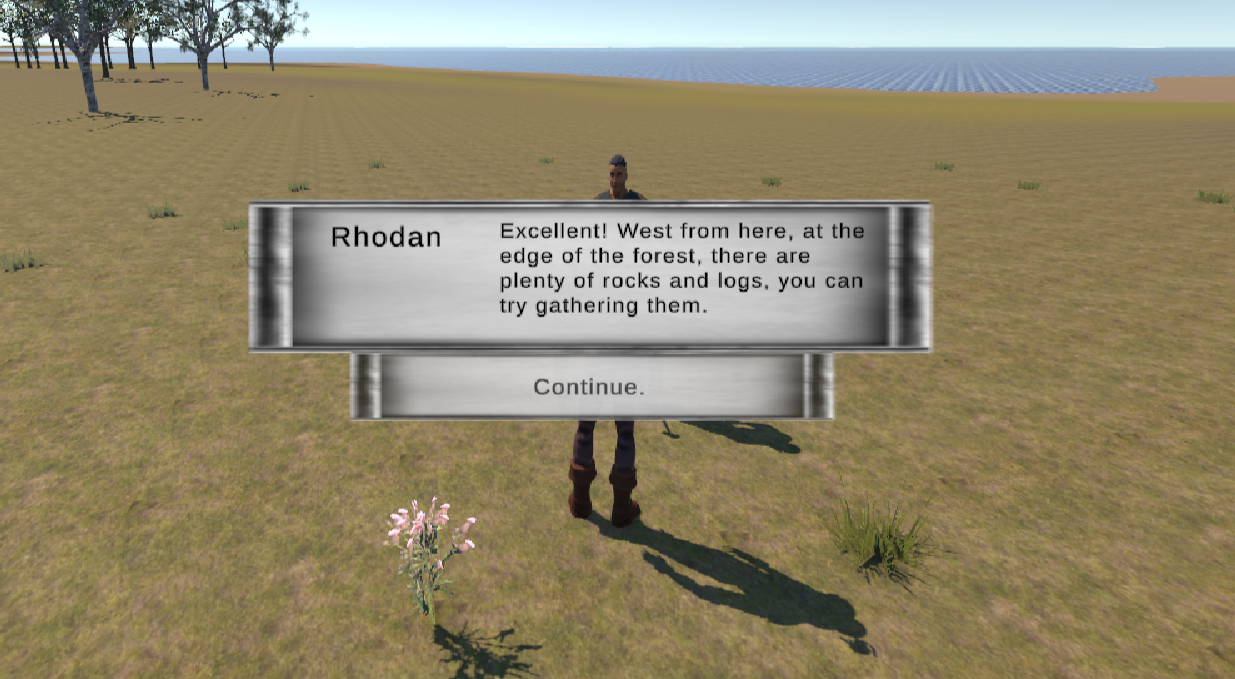
\includegraphics[width=1\textwidth]{images/rozgrywka/rhodan4.png}
    \caption{Kadr z dialogu z Rhodanem z wytycznymi odnośnie zbierania zasobów.}
\end{figure}

Po zebraniu zasobów wraca porozmawiać z Rhodanem. Dowiaduje się od niego, że gdy mu wskaże odpowiednie do budowy namiotu
miejsce, to postać podejdzie i go wybuduje. Tak jak został poinstruowany, gracz wybiera wystarczająco płaskie miejsce,
które nie jest zajęte przez jakiś inny obiekt. Po zatwierdzeniu Rhodan podbiega do powstałego fundamentu i rozpoczyna
bydowę, wspomagając się młotkiem. Gdy mężczyzna skończył pracę gracz może podejść z nim porozmawiać i odebrać swoją
nagrodę.

\begin{figure}[h!]
    \centering
    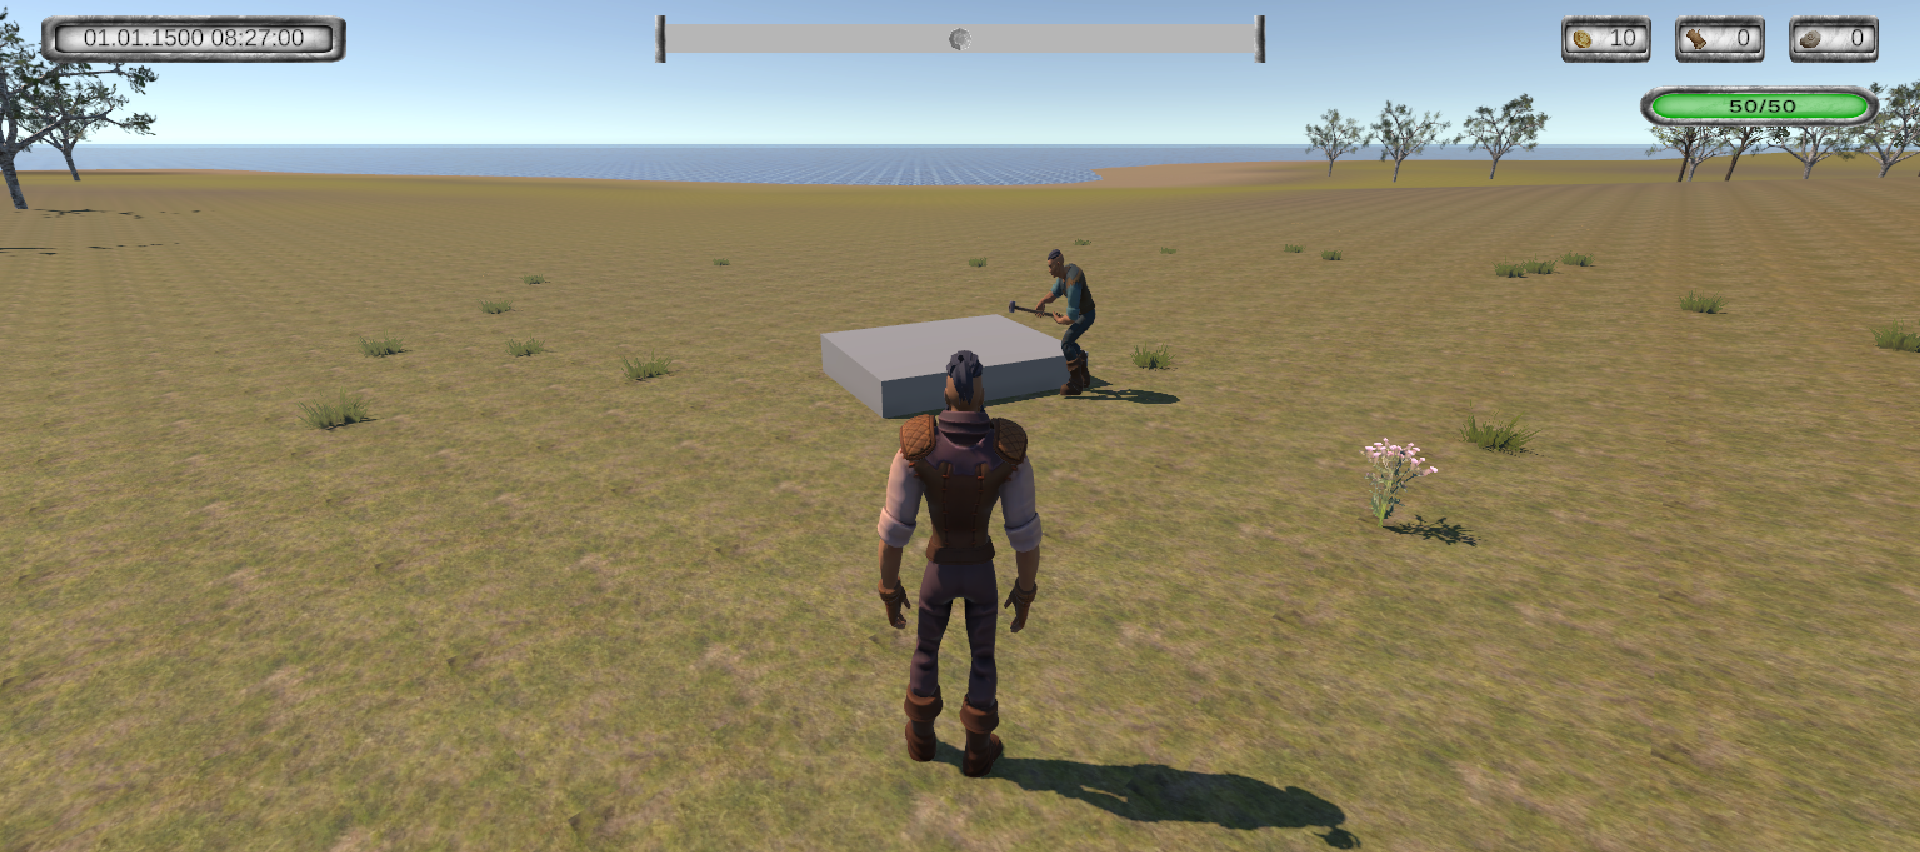
\includegraphics[width=1\textwidth]{images/rozgrywka/rhodan9.png}
    \caption{Kadr z gry, na którym widać budującego Rhodana.}
\end{figure}